\documentclass[10.5pt,a4paper]{article} 
\usepackage[utf8]{inputenc}  

\usepackage[scaled]{helvet}
\renewcommand\familydefault{\sfdefault} 
\usepackage[T1]{fontenc}
\usepackage[light]{merriweather} 
%\usepackage{ulem}
\usepackage{setspace} 
\usepackage[hang]{footmisc} 
\renewcommand{\footnotesize}{\scriptsize} 
\usepackage[hyphens]{url}\urlstyle{same} 
\usepackage[colorlinks = true,
            linkcolor = black,
            urlcolor  = blue,
            citecolor = black,
            anchorcolor = black]{hyperref}
% e-mail
\usepackage{etoolbox}
\makeatletter
\newcommand\myemail[3]{%                %\newcommand\tpj@compose@mailto[3]{%
\edef\@tempa{mailto:#1?subject=#2 }%
\edef\@tempb{\expandafter\html@spaces\@tempa\@empty}%
\href{\@tempb}{#3}}
\catcode\%=11
\def\html@spaces#1 #2{#1%20\ifx#2\@empty\else\expandafter\html@spaces\fi#2}
\catcode\%=14
\makeatother
% Colour
\usepackage[svgnames]{xcolor}
\definecolor{rstudio}{HTML}{4b84b7}
\definecolor{cloud}{HTML}{e4eef8}

\Urlmuskip=0mu plus 1mu\relax 
\usepackage[margin=2.5cm]{geometry} 
\usepackage{fancyhdr} % Required for modifying headers and footers
\fancyhead[L]{} % Top left header
\fancyhead[R]{} % Top right header
\renewcommand{\headrulewidth}{1.4pt} % Rule under the header
\fancyfoot[C]{\textbf{\thepage}} % Bottom center footer
\renewcommand{\footrulewidth}{1.4pt} % Rule under the footer
\pagestyle{fancy} % Use the custom headers and footers throughout the document


\usepackage{lipsum,afterpage}
\usepackage{dirtytalk} 
\usepackage{longtable}
\usepackage{adjustbox}
\usepackage{apacite}
\usepackage{natbib}
\usepackage{tkz-euclide}
\usetikzlibrary{calc}
\usepackage{pgfplots}
\pgfplotsset{compat=1.11}
\usepackage {parskip}
\usepackage{epigraph}
\usepackage{graphicx}
\graphicspath{ {images/} }
\pagenumbering{arabic} 
\usepackage{ntheorem}
\newtheorem{hyp}{Hypothesis}
\newtheorem{subhyp}{Hypothesis}[hyp]
\renewcommand\thesubhyp{\thehyp.\alph{subhyp}}
\usepackage{caption}
\usepackage{subcaption}
\usepackage{float}
\usepackage[bf,sf]{titlesec}

\renewcommand{\refname}{Bibliography}
%\setcounter{secnumdepth}{0}
\usepackage[autostyle]{csquotes}
\usepackage{enumitem} % to remove vspace for itemize with [noitemsep]

\usepackage{listings}
\lstset{language=R,
    basicstyle=\small\ttfamily,
    stringstyle=\color{DarkGreen},
    otherkeywords={!,!=,~,$,*,\&,\%/\%,\%*\%,\%\%,<-,<<-,_,/},
    morekeywords={TRUE,FALSE},
    deletekeywords={data,frame,length,as,character},
    keywordstyle=\color{Chocolate},
    commentstyle=\color{DarkSlateGrey}
}

\usepackage{xparse}
\ExplSyntaxOn

\makeatletter
\NewDocumentCommand{\multicitep}{m}
 {
  \NAT@open
  \mjb_multicitep:n { #1 }
  \NAT@close
 }
\makeatother
\seq_new:N \l_mjb_multicite_in_seq
\seq_new:N \l_mjb_multicite_out_seq
\seq_new:N \l_mjb_cite_seq

\cs_new_protected:Npn \mjb_multicitep:n #1
 {
  \seq_set_split:Nnn \l_mjb_multicite_in_seq { ; } { #1 }
  \seq_clear:N \l_mjb_multicite_out_seq
  \seq_map_inline:Nn \l_mjb_multicite_in_seq
   {
    \mjb_cite_process:n { ##1 }
   }
  \seq_use:Nn \l_mjb_multicite_out_seq { ;~ }
 }

\cs_new_protected:Npn \mjb_cite_process:n #1
 {
  \seq_set_split:Nnn \l_mjb_cite_seq { , } { #1 }
  \int_compare:nTF { \seq_count:N \l_mjb_cite_seq == 1 }
   {
    \seq_put_right:Nn \l_mjb_multicite_out_seq
     { \citeauthor{#1},~\citeyear{#1} }
   }
   {
    \seq_put_right:Nx \l_mjb_multicite_out_seq
     {
      \exp_not:N \citeauthor{\seq_item:Nn \l_mjb_cite_seq { 1 }},~
      \exp_not:N \citeyear{\seq_item:Nn \l_mjb_cite_seq { 1 }},~
      \seq_item:Nn \l_mjb_cite_seq { 2 }
     }
   }
 }
\ExplSyntaxOff

\title{\textbf{\emph{RStudio Cloud}} pour les nuls}
\author{William Poirier, Université Laval}
\date{POL-2000 -- Automne 2021}

\begin{document} 

% ----------------------------------------------------------------
\begin{titlepage}
\newgeometry{left=7.5cm} %defines the geometry for the titlepage
\pagecolor{rstudio}
\noindent

\includegraphics[width=13.6cm]{_graphs/cloud.jpg}\\[-1em]
\color{cloud}
\makebox[0pt][l]{\rule{1.4\textwidth}{2pt}}
\par
\noindent
\color{white}
\textbf{Université Laval}
\vfill
\noindent
{\huge\textbf{\emph{RStudio Cloud}} pour les nuls}
\vskip\baselineskip
\noindent
POL-2000 -- Automne 2021
\end{titlepage}
\restoregeometry % restores the geometry
\nopagecolor% Use this to restore the color pages to white
% ----------------------------------------------------------------

\tableofcontents

\pagebreak

\section{C'est quoi R?}
Bonjour et bienvenue au cours Pol-2000, ce tutoriel sera votre guide de démarrage ainsi qu'un document de référencement tout au long du cours\footnote{Tutoriel basé sur le travail de Vincent Arel-Bundock, Yannick Dufresne, et Florence Vallée-Dubois}. Le cours ayant pour objectif d'introduire les étudiants de sciences politiques aux méthodes quantitatives et à l'analyse causale en science sociale, nous avons cru bons de vous initier au langage de programmation R. N'ayez crainte, c'est plus simple qu'il n'y paraît et vous en tirerez beaucoup d'avantages. 

Pour la petite histoire, la première version de \textbf{R} a été publiée en 1995 par Ross Ihaka et Robert Gentleman, mais le langage s'inspire des travaux de John Chambers aux laboratoires Bell dans les années 1970. Aujourd'hui, \textbf{R} est un outil d'analyse statistique populaire, tant dans le secteur privé que dans le monde universitaire. \textbf{R} est-ce que l'on appelle un \textit{logiciel libre}, ce qui signifie que son code source est ouvert. Ceci permet à des utilisateurs bénévoles de développer des \textit{packages} (micrologiciel ou librairie de fonctions) qui sont ensuite rendu disponible à la communauté (pour la plupart gratuitement). Ceci fait de \textbf{R} un outil puissant,flexible et public, ce qui le rend particulièrement adapté à la méthode scientifique. 

Le reste du document vous permettra de vous familiariser avec \textbf{R} et son environnement de travail. Nous encourageons donc sa lecture attentive.

\section{R vs RStudio vs RStudio Cloud}

Une distinction importante à effectuer est la différence entre le langage \textbf{R} et l'\textit{IDE}\footnote{\emph{Itegrated development environment} ou environnement de développement intégré.} \textbf{RStudio}. L'\textit{IDE} a pour fonction principale de recevoir le code et de le compiler. En d'autres mots, \textbf{R} c'est la langue que l'on écrit et le papier c'est l'\textit{IDE}. Plusieurs \textit{IDE} existent et il est facile de se perdre dans leurs différents paramètres et fonctionnalités. C'est pourquoi nous imposons l'utilisation de \textbf{RStudio} ou, à proprement parler, de \textbf{RStudio Cloud}. \textbf{RStudio Cloud} est une reproduction de l'environnement \textbf{RStudio} en ligne. De cette façon, tous les étudiants ont accès au même environnement de travail, peu importe l'ordinateur utilisé.  

Ainsi, dans le cadre du cours, les étudiants utiliserons le langage de programmation \textbf{R} à partir de l'environnement \textbf{RStudio Cloud}. Cette distinction s'affinera au cours de la session, n'ayez crainte. Pour les plus curieux d'entre-vous, de nombreuses ressources, francophone et anglophone, existent sur internet :

\begin{itemize}
  \item \href{https://stackoverflow.com}{Stackoverflow}
    \begin{itemize}
      \item Google est le meilleur ami des programmeurs. Si vous rencontrez un problème, Google vous fournira sans doute la solution sous la forme d'un \textit{post} sur Stackoverflow. Il s'agit d'un site répertoriant les questions d'utilisateurs concernant la plupart des langages de programmation, incluant \textbf{R}. À la manière du logiciel libre, ce sont les autres utilisateurs du site qui se chargent de répondre avec grande précision. C'est vraiment un outil important. 
    \end{itemize}
  \item \href{https://www.r-bloggers.com}{r-bloggers}
    \begin{itemize}
      \item Pour être informé sur les nouveaux développements de R et de RStudio. Encore une fois, il s'agit d'un point de rencontre de la communauté.
    \end{itemize}
  \item \href{https://www.coursera.org}{Coursera}
    \begin{itemize}
      \item Site de formation en ligne. Les cours ont le format de cours universitaires, mais avec la version gratuite: pas besoin de suivre l’entièreté des plans de cours (ni de remettre les travaux).
    \end{itemize}
  \item \href{https://www.datacamp.com}{DataCamp}
    \begin{itemize}
      \item Similaire à Coursera, DataCamp se concentre sur des exercices pratiques en \textbf{Python}, \textbf{R} et \textbf{SQL}. Avec une approche très pratique, c'est un bon moyen d'accélérer l'intégration de connaissances techniques. 
    \end{itemize}
\item \href{https://www.datanovia.com/en/}{Datanovia}
    \begin{itemize}
      \item Sous forme de tutoriel et de blogue, Datanovia est une excellente source d'information bilingue, spécialement lorsqu'il s'agit de visualisation de données.
    \end{itemize}
\end{itemize}

\section{RStudio Cloud -- La base}
  \subsection{Connexion}
  Dans le cadre du cours, nous utiliserons un espace de travail commun. Pour y accéder, veuillez d'abords vous créer un compte \textbf{RStudio Cloud} en cliquant \href{https://login.rstudio.cloud/register?redirect=https\%3A\%2F\%2Fclient.login.rstudio.cloud\%2Foauth\%2Flogin\%3Fshow_auth\%3D0\%26show_login\%3D0\%26show_setup\%3D0}{\textbf{ici}}. Une fois que votre compte est créé, cliquez \href{https://can01.safelinks.protection.outlook.com/?url=https\%3A\%2F\%2Flogin.rstudio.cloud\%2Finvite\%3Fspace_name\%3DPOL\%2B2000-Z\%2BM\%25C3\%25A9thodes\%2Bquantitatives\%26code\%3D9tltN\%252ByVLqitCL1rVgCB\%252F\%252B0V8rk0Wtqxp\%252Fl6uW8J&amp;data=04\%7C01\%7Cwilliam.poirier.1\%40ulaval.ca\%7C9119a0b3a3fa4119007208d987439312\%7C56778bd56a3f4bd3a26593163e4d5bfe\%7C1\%7C0\%7C637689547430424200\%7CUnknown\%7CTWFpbGZsb3d8eyJWIjoiMC4wLjAwMDAiLCJQIjoiV2luMzIiLCJBTiI6Ik1haWwiLCJXVCI6Mn0\%3D\%7C0&amp;sdata=EMbletbv2\%2Bu9\%2FKSqkqJbRadybcaee2t2S2\%2F8MNRvJgQ\%3D&amp;reserved=0}{\textbf{ici}} pour accéder à l'environnement du cours. Tous les exercices et travaux pratiques s’y trouvent.
  
\begin{figure}[H]
\centering
\begin{subfigure}{.5\textwidth}
  \centering
  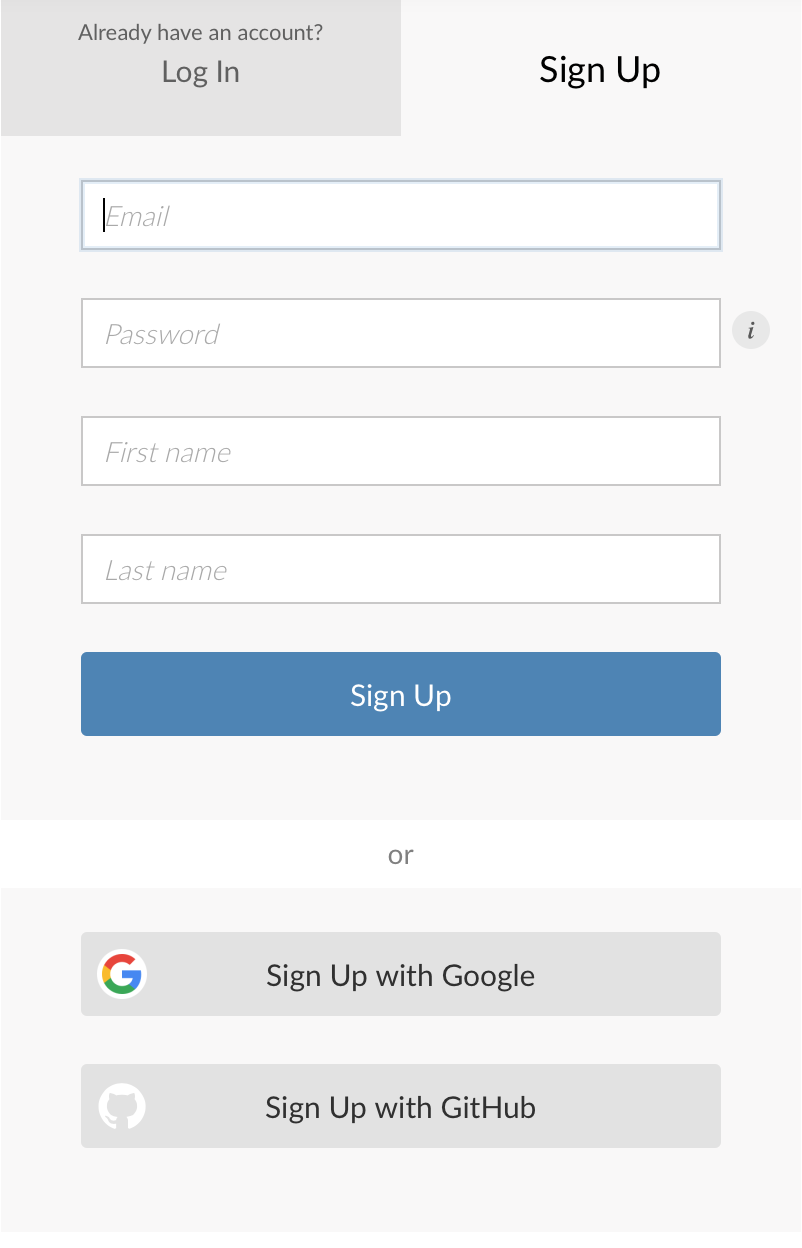
\includegraphics[width=1\linewidth]{_graphs/login.png}
  \caption{Création du compte}
  \label{login}
\end{subfigure}%
\begin{subfigure}{.5\textwidth}
  \centering
  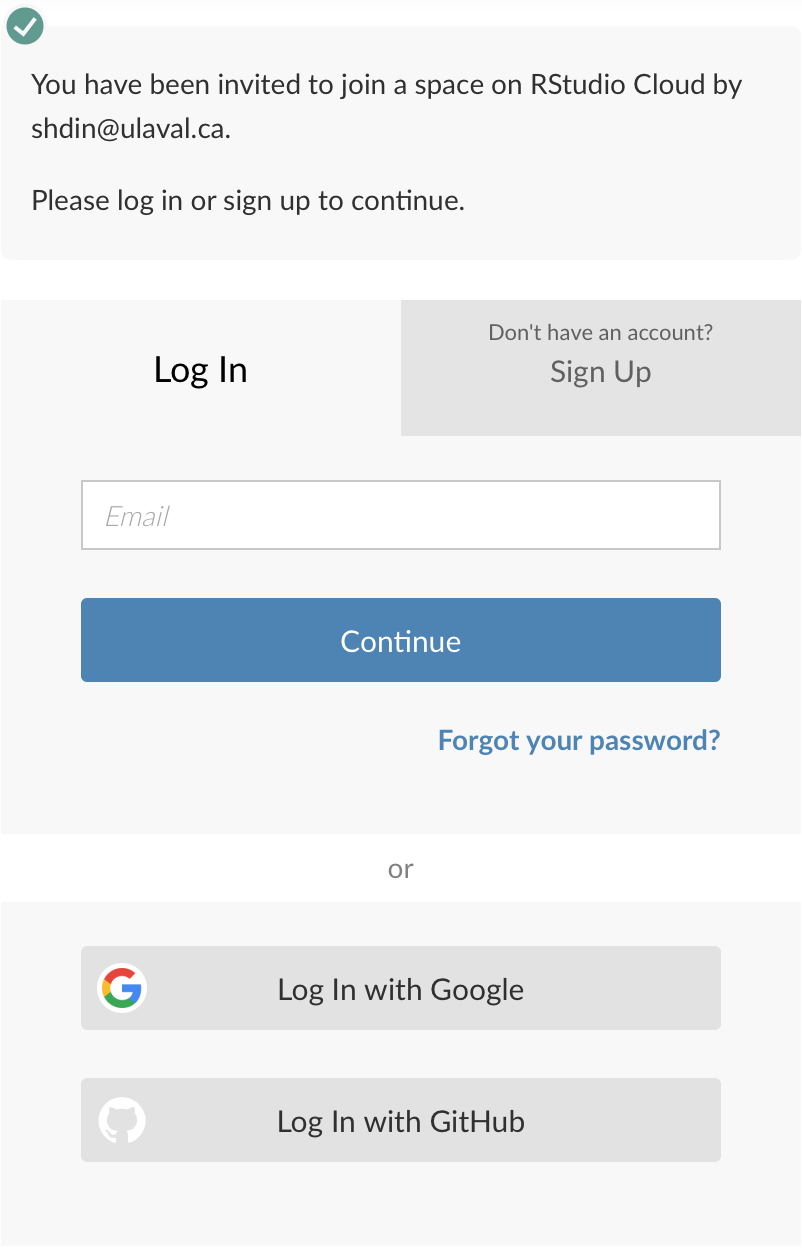
\includegraphics[width=1\linewidth]{_graphs/workspace.png}
  \caption{Inscription à l'environnement}
  \label{workspace}
\end{subfigure}
\caption{Connexion à \textbf{RStudio Cloud}}
\label{connexion}
\end{figure}
  
  \subsection{Interface}
  \textbf{RStudio Cloud} a deux interfaces, l'interface des espaces de travail et l'interface des projets. L'interface des espaces de travail est la première chose que vous rencontrez en vous connectant à \textbf{RStudio Cloud}. C'est ce qui vous permet de vous déplacer d'un projet à l'autre et d'un espace de travail à l'autre. La section \emph{menu} de cette interface offre aussi plusieurs liens à des ressources externes sur 1) l'utilisation de \textbf{RStudio Cloud}, 2) l'utilisation de \textbf{R} et 3) de ses \emph{packages} les plus populaires. Les figures \ref{home} et \ref{homeMenu} présentent un aperçu de l'interface des espaces de travail de \textbf{RStudio Cloud} et ses principaux points d'intérêt.
  
\begin{figure}[H]
  \centering
  \fbox{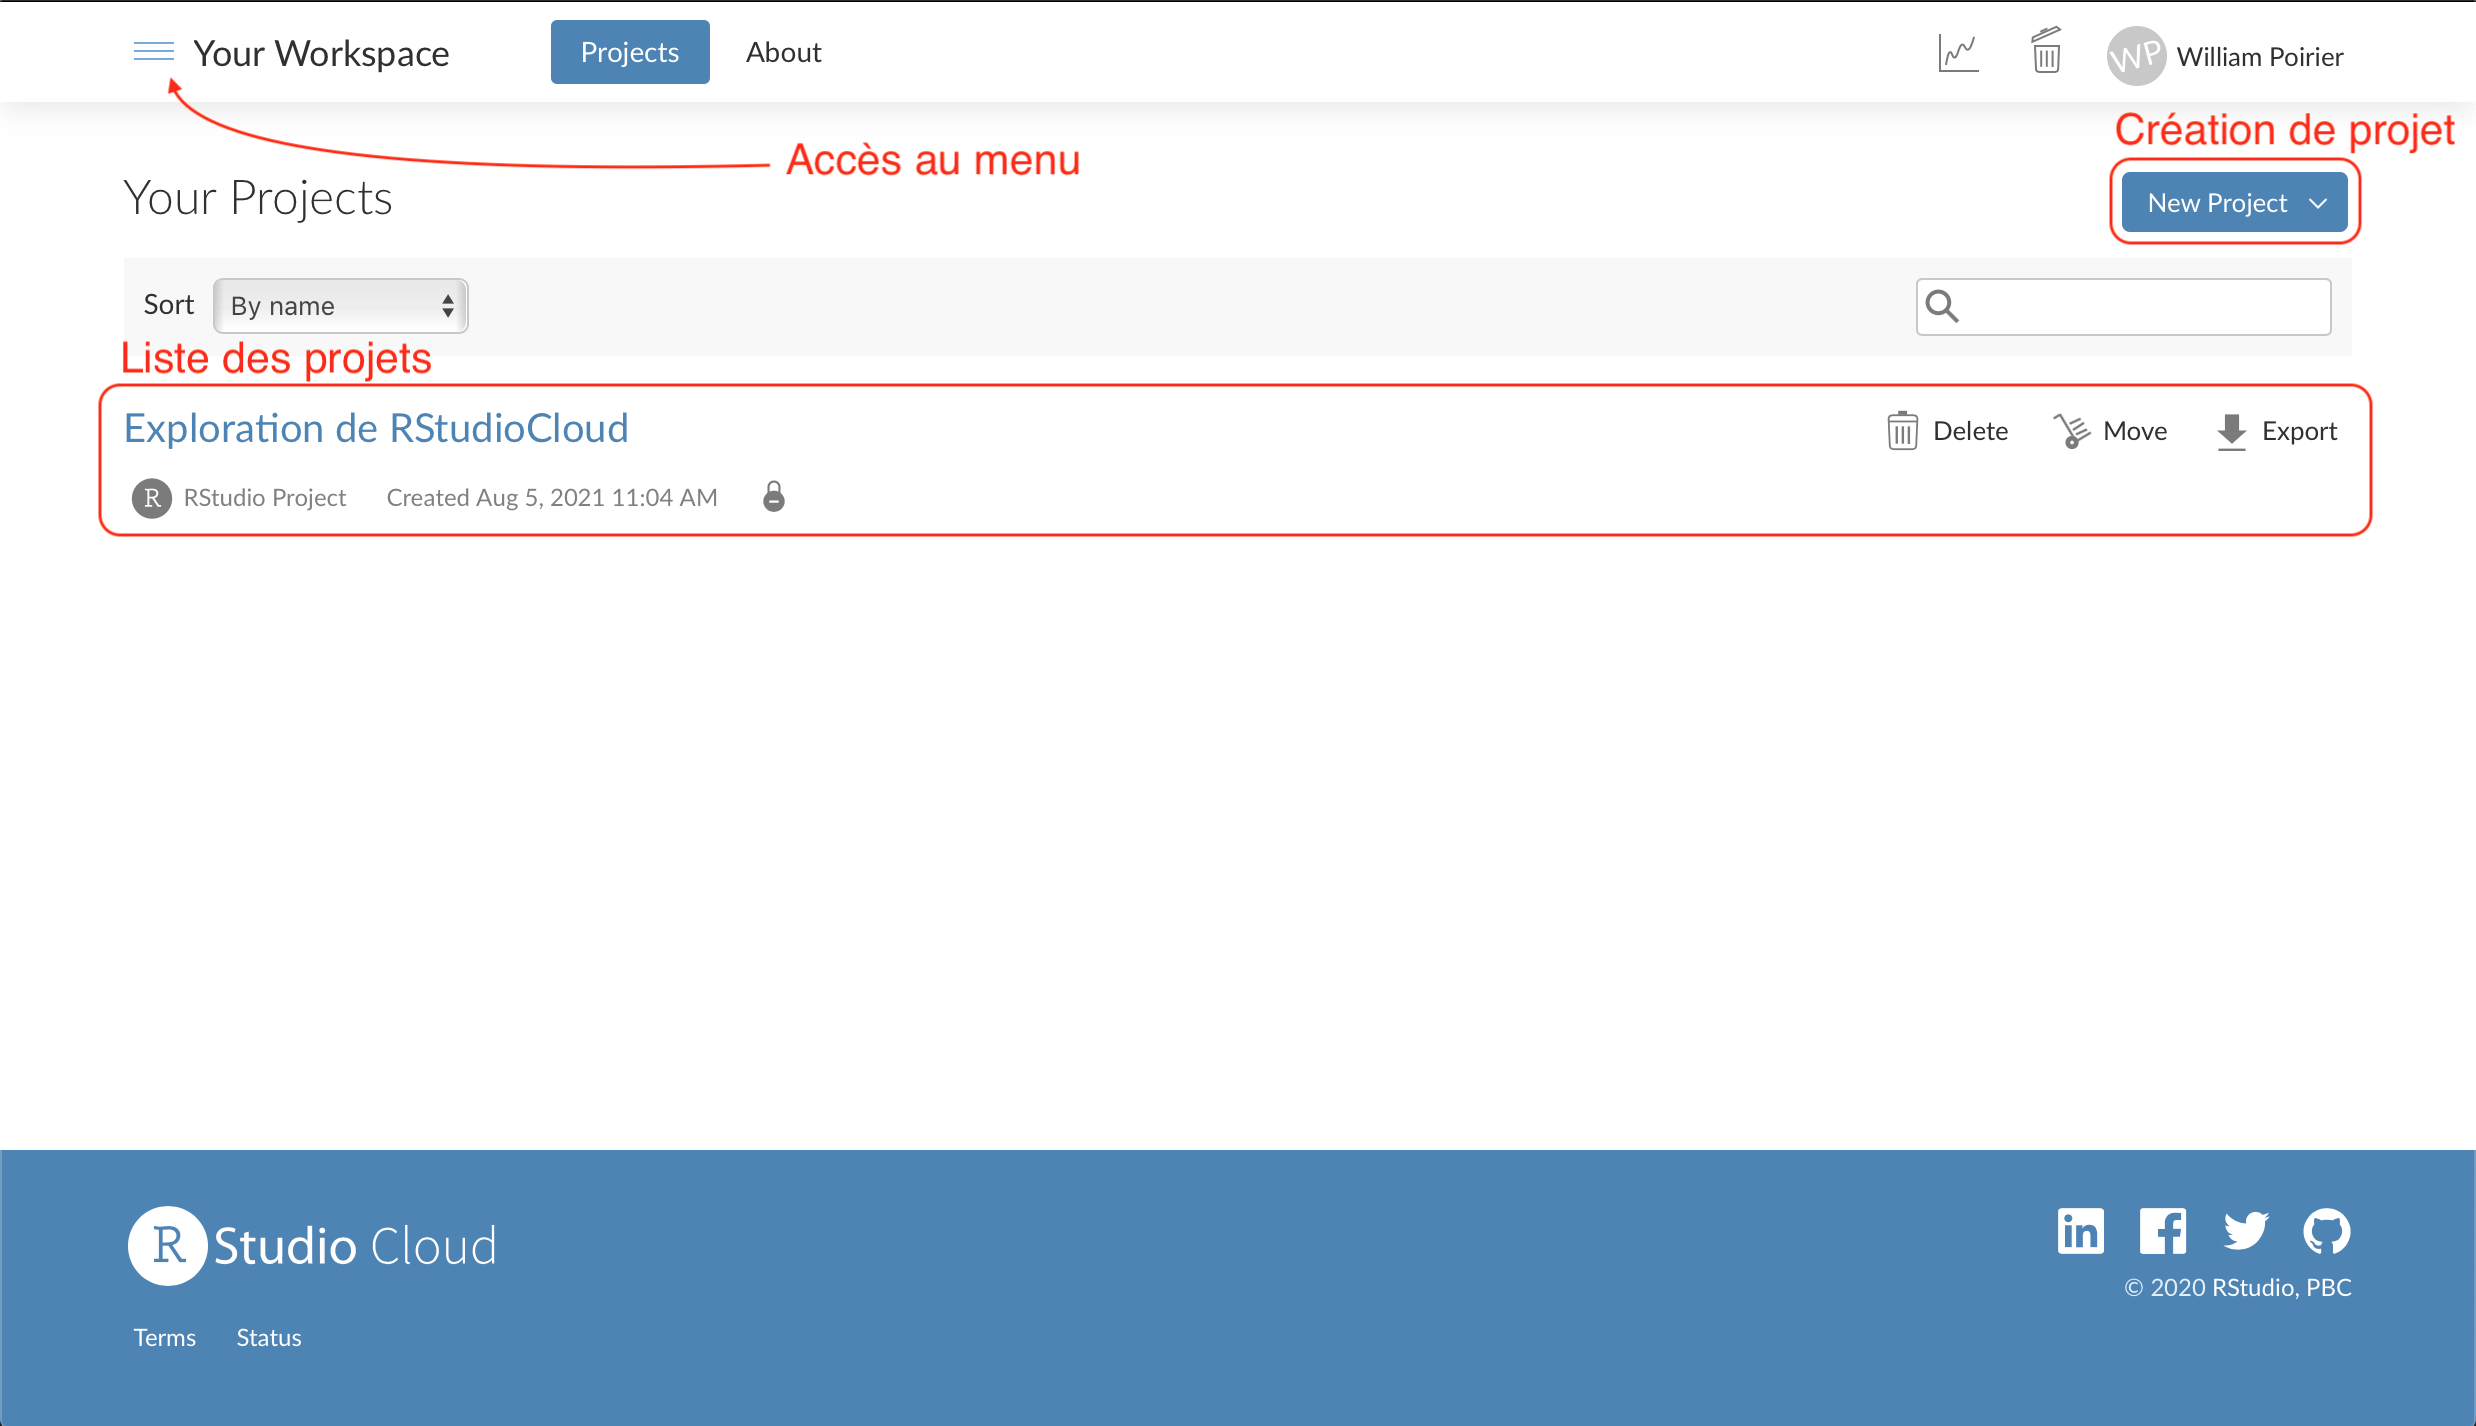
\includegraphics[width=1\linewidth]{_graphs/firstpage.png}}
  \caption{Page d'accueil}
  \label{home}
\end{figure}

\begin{figure}[H]
  \centering
  \fbox{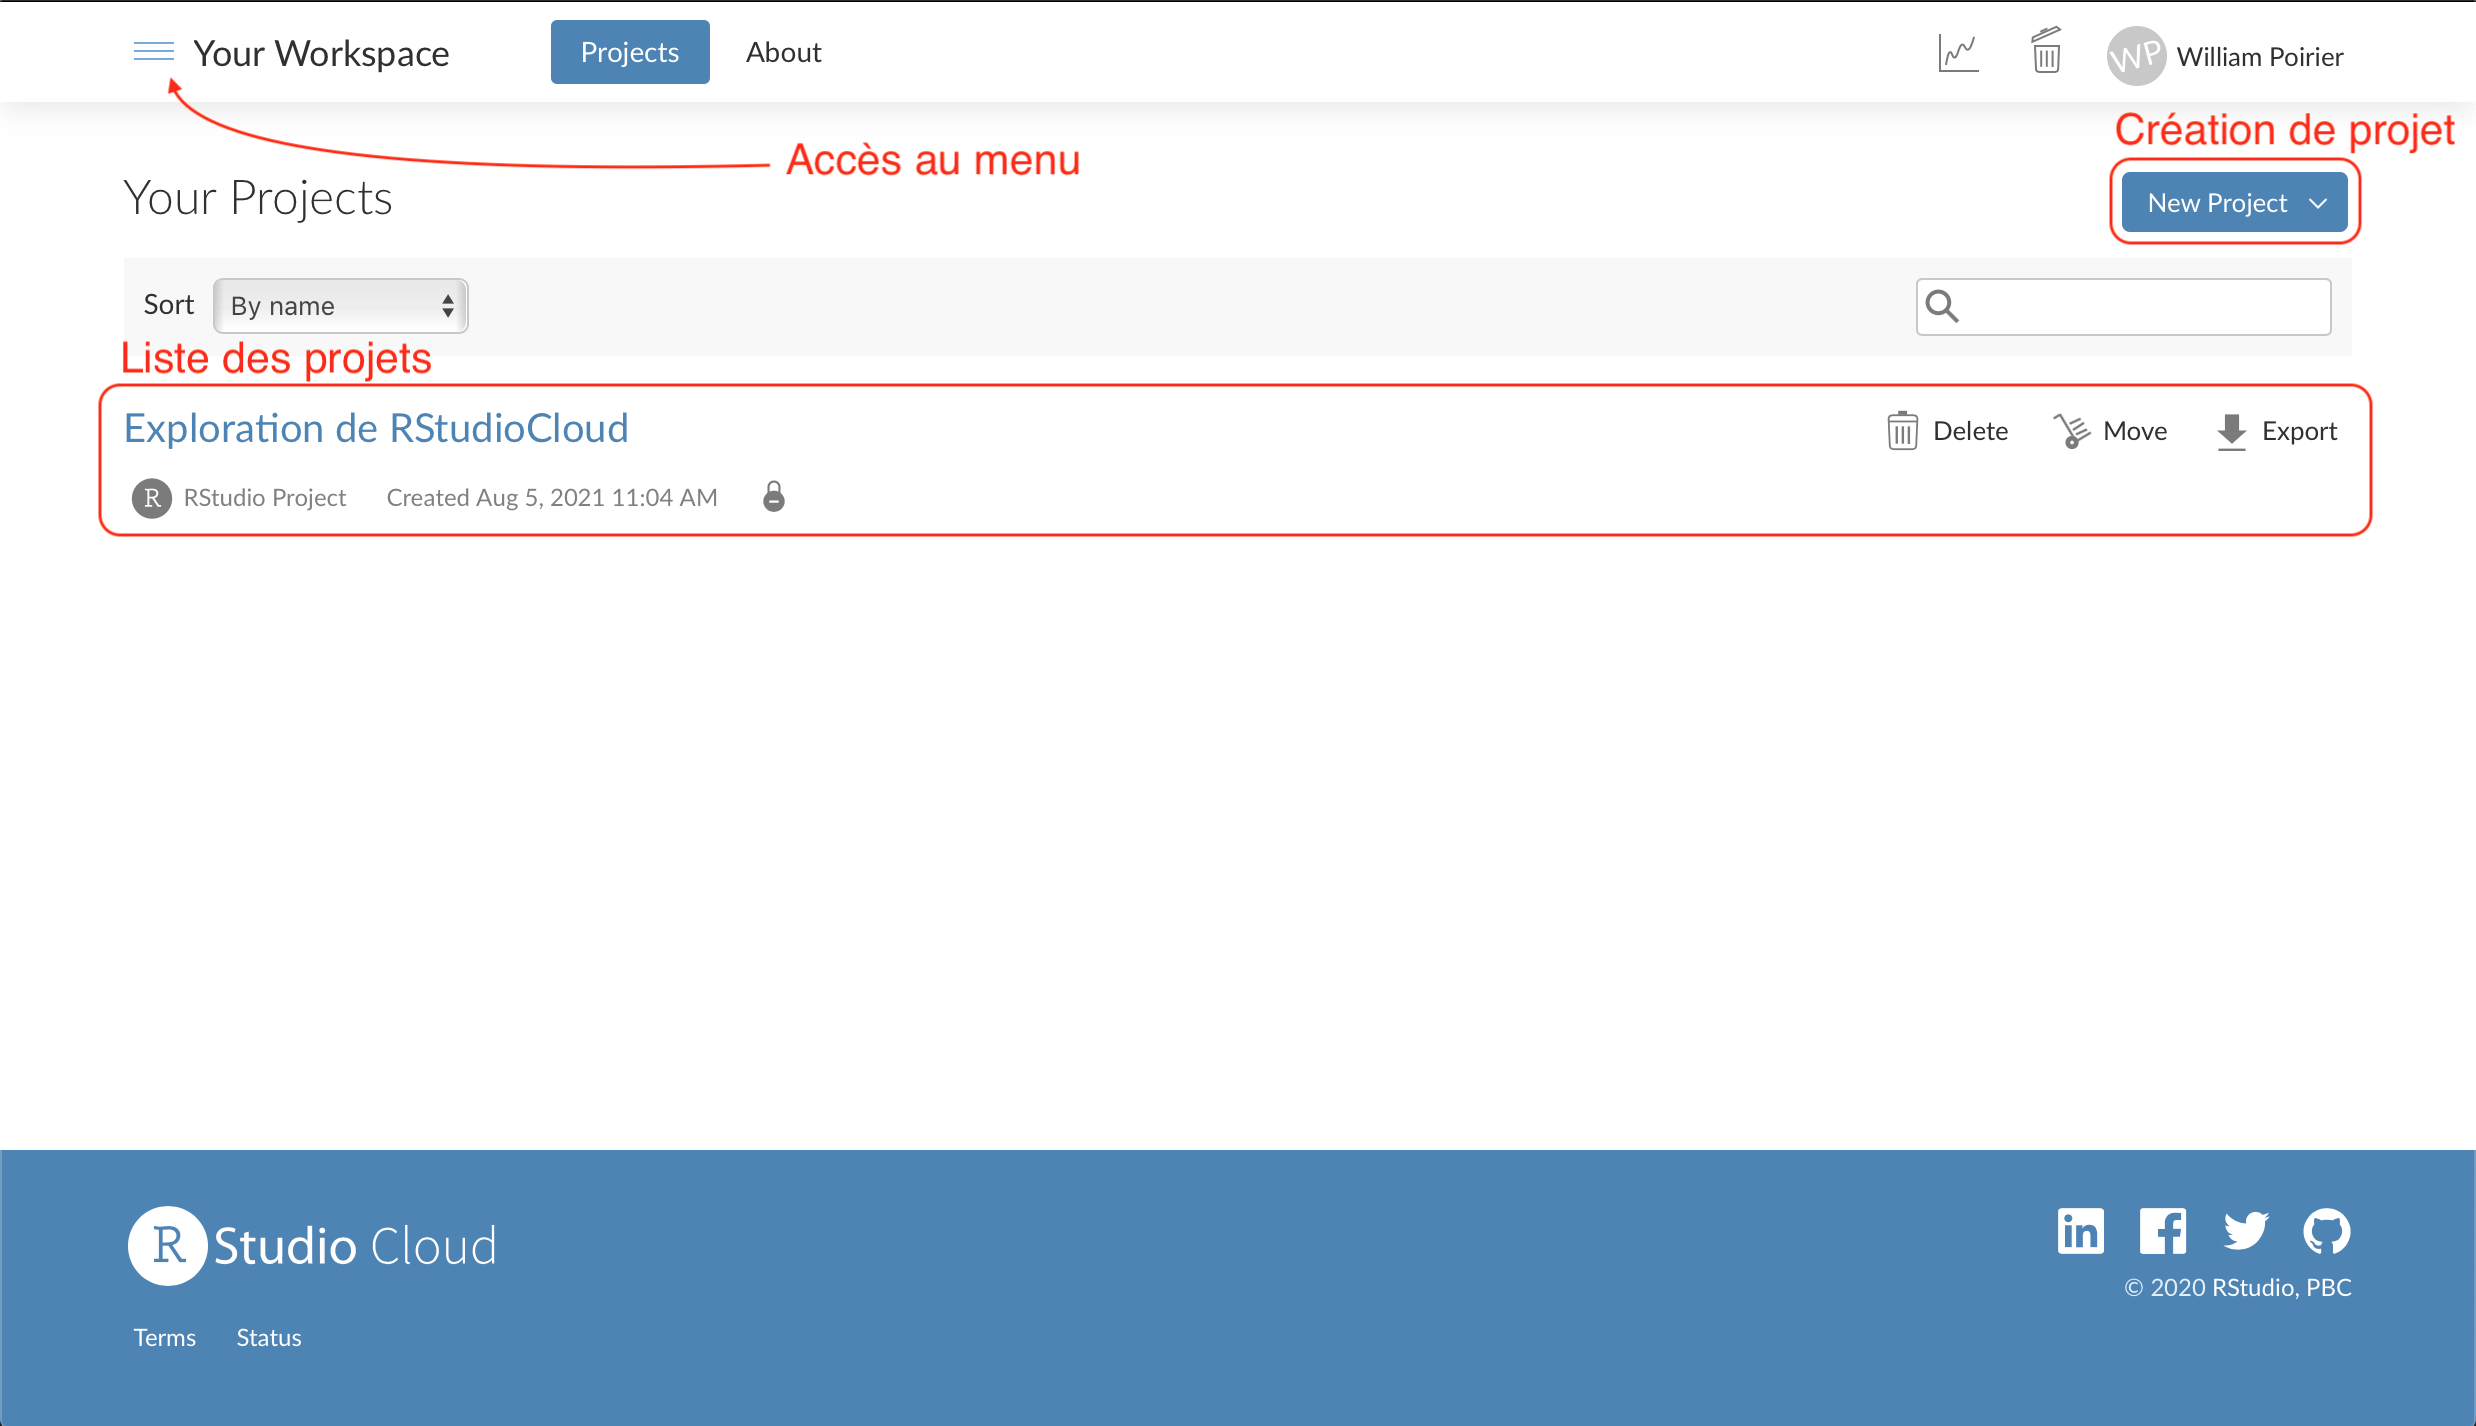
\includegraphics[width=1\linewidth]{_graphs/firstpage.png}}
  \caption{Menu d'accueil}
  \label{homeMenu}
\end{figure}

  La seconde interface est celle qui nous intéresse le plus, c'est où vous écrirez et exécuterez votre code. La figure \ref{rstudio1} présente les points d'intérêts les plus importants. L'\emph{environnement} contiendra les bases de données que vous importerez ainsi que tous les objets créés lors de la session\footnote{Ici, \emph{session} fait référence à la période de travail sur \textbf{RStudio Cloud}.}. Vous pouvez avoir accès à vos dossiers, les librairies utilisées, un aperçus des graphiques produits ainsi qu'à de l'aide dans la fenêtre en bas à droite. La plus grande fenêtre par défaut est celle contenant la console. La \textbf{console} est un environnement d'exécution directe. En d'autres mots, vous pouvez y écrire des commendes qui seront exécutées immédiatement. C'est utile pour faire des tests et exécuter de petite manipulation. Or, la \textbf{console} n'enregistre pas la suite de commende que vous lui demander de faire, ce n'est pas son rôle. Pour ce faire, il faut ouvrir l'\textbf{éditeur} tel que spécifié par la figure \ref{rstudio1}. L'\textbf{éditeur} c'est où l'on écrit un script (une suite de commandes permettant d'atteindre un but quelconque, comme la production d'un graphique) afin qu'il puisse être enregistré et réutilisé.  
  
\begin{figure}[H]
  \centering
  \fbox{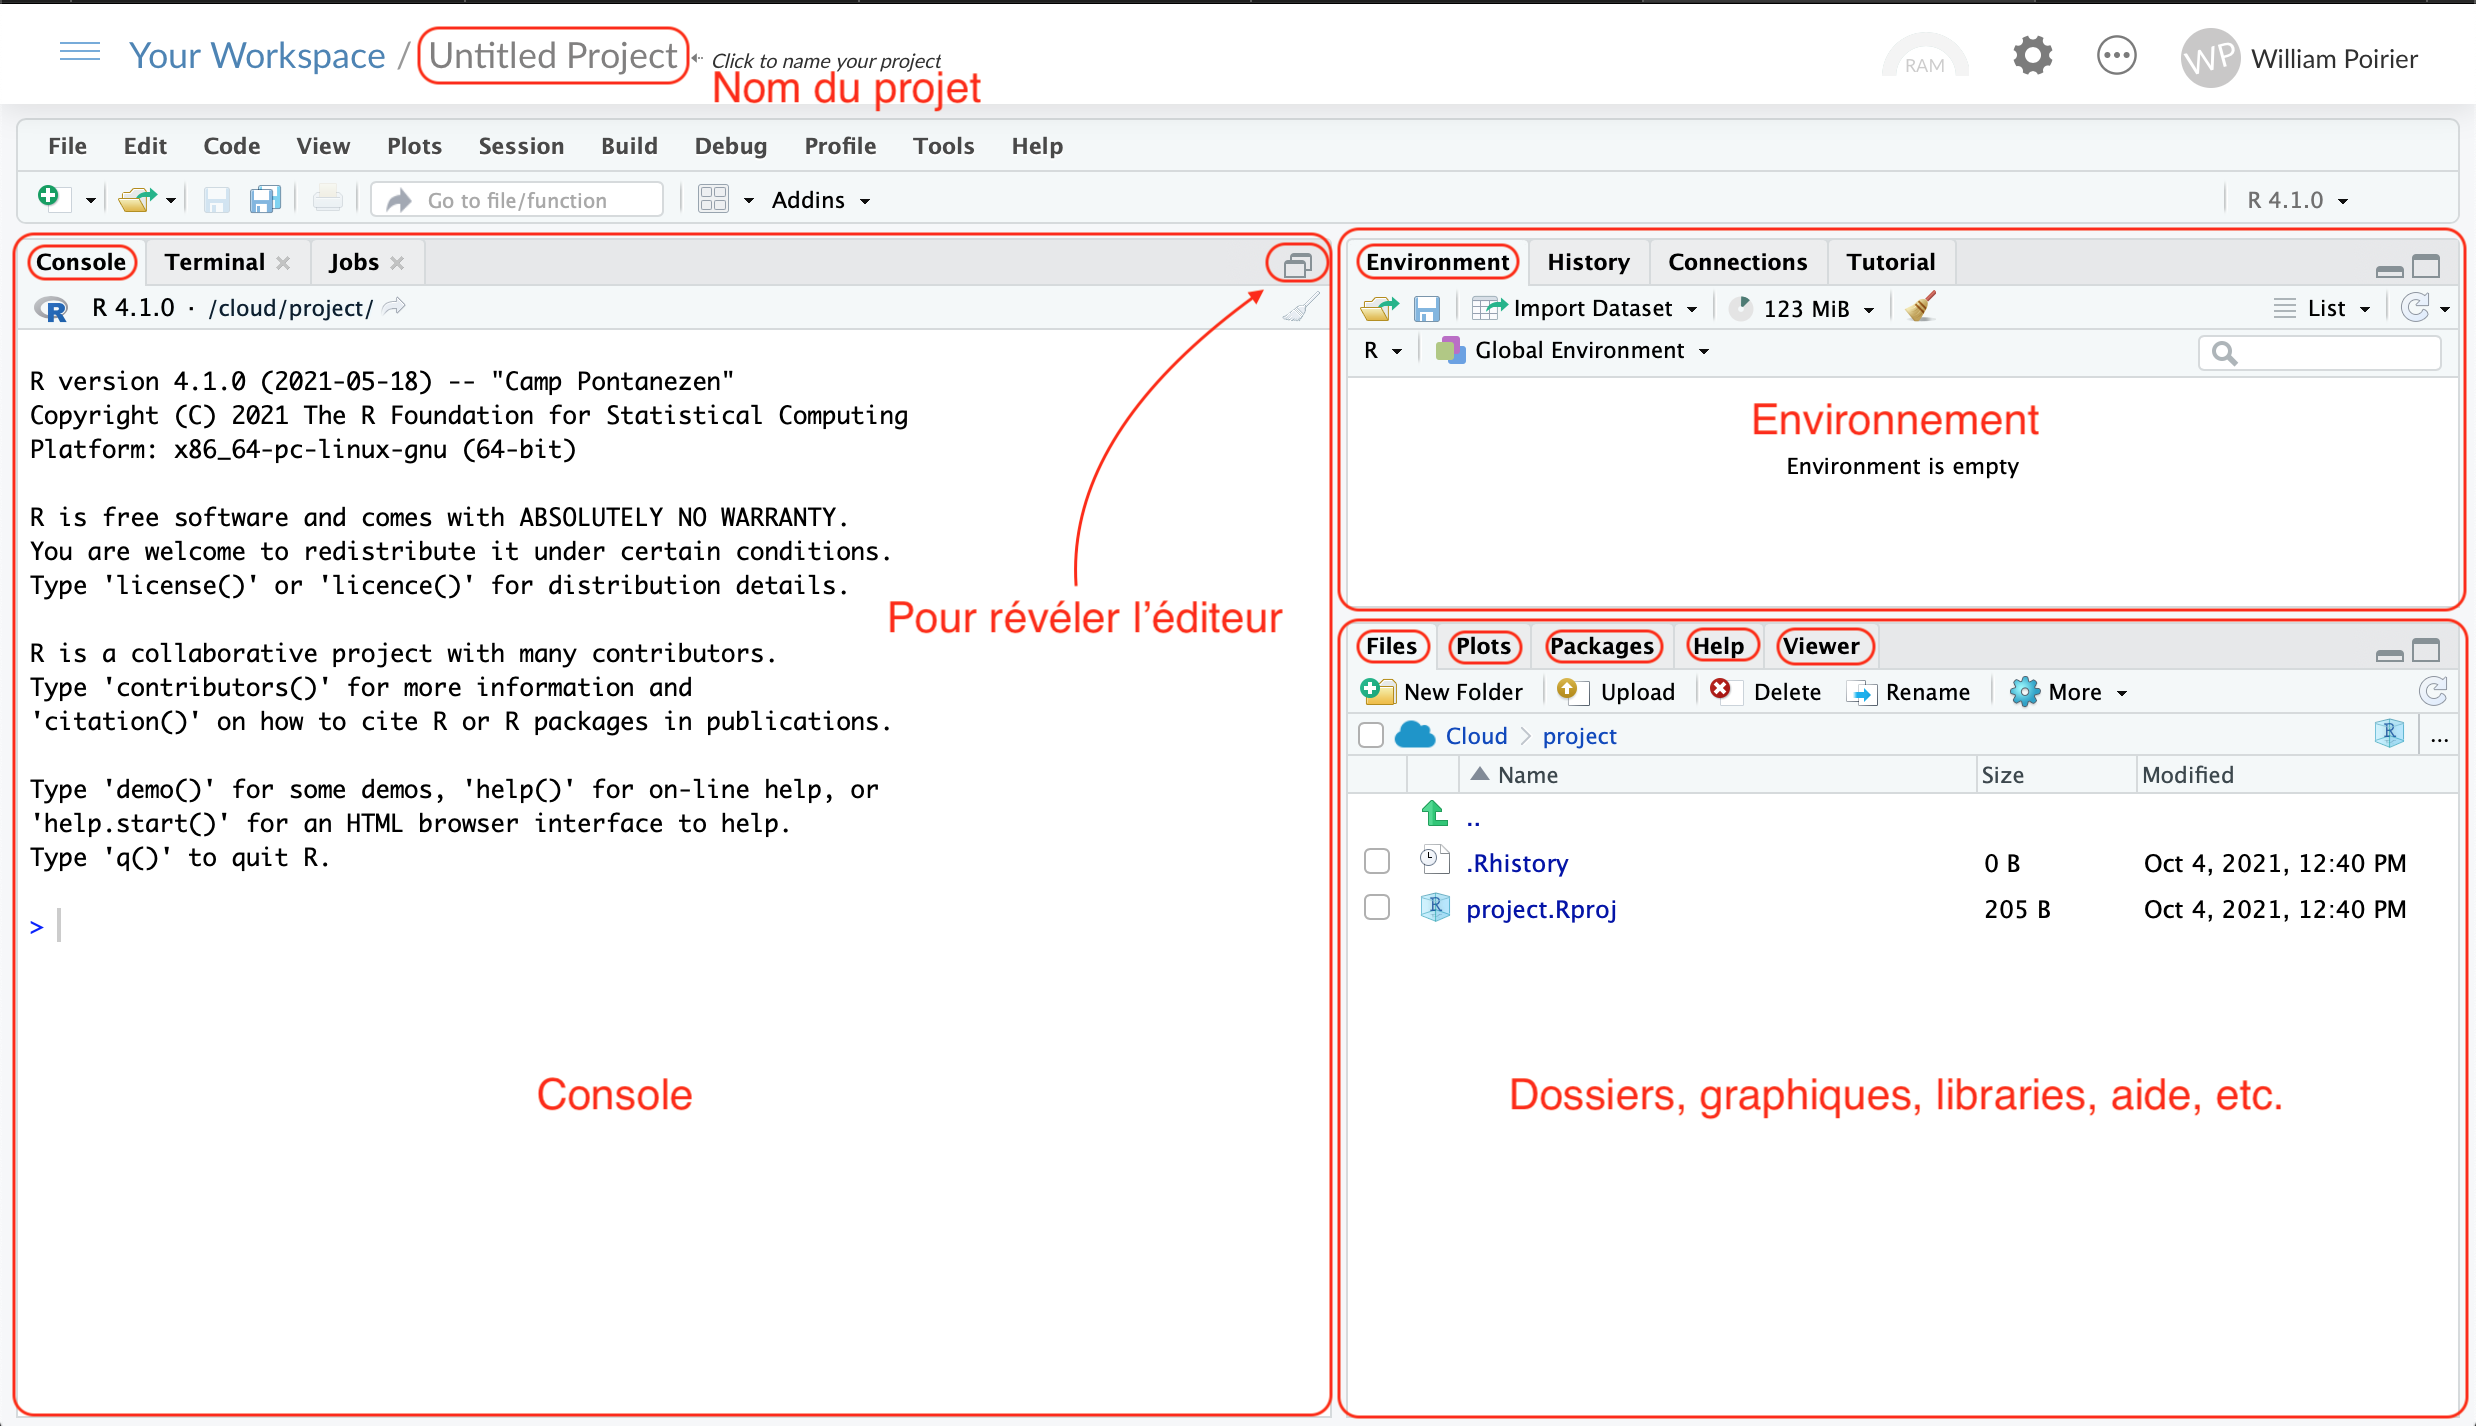
\includegraphics[width=0.98\linewidth]{_graphs/rstudio1.png}}
  \caption{État par défaut}
  \label{rstudio1}
\end{figure}

\begin{figure}[H]
  \centering
  \fbox{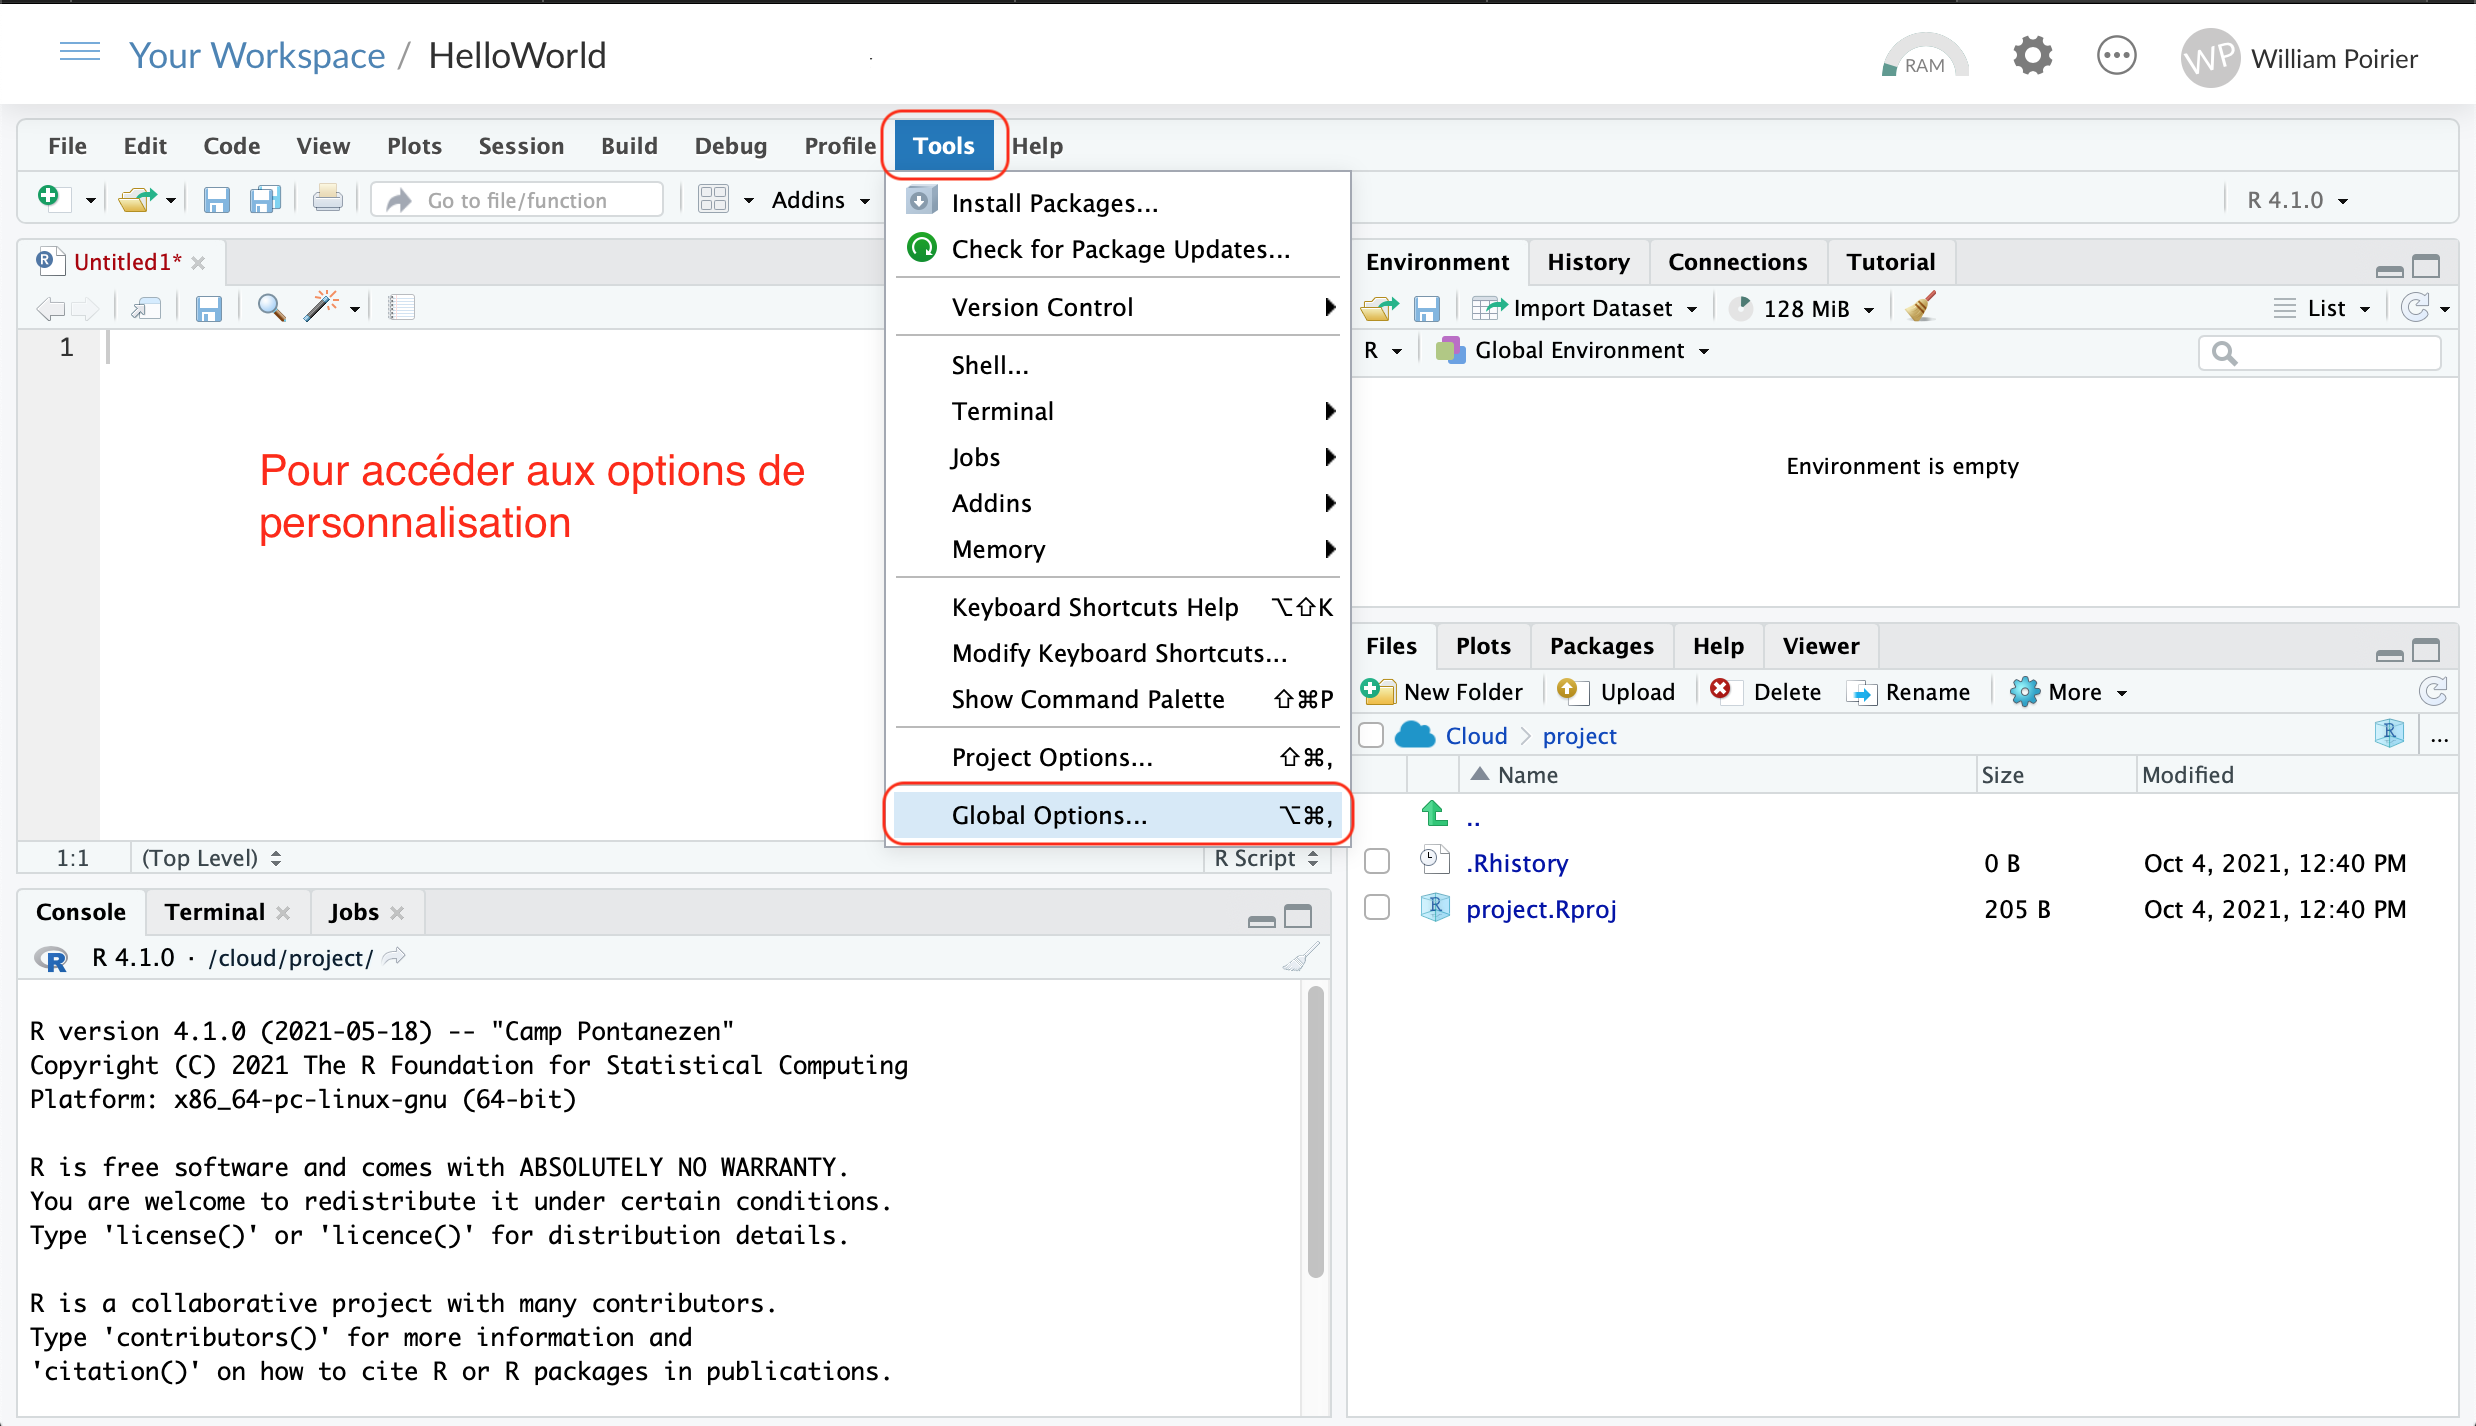
\includegraphics[width=0.98\linewidth]{_graphs/rstudio2.png}}
  \caption{Début de la personnalisation}
  \label{rstudio2}
\end{figure}

Avant d'entrer dans la syntaxe d'utilisation de \textbf{R}, je recommande fortement la personnalisation de votre environnement. Non seulement cela vous permettra d'avoir une expérience esthétique plus agréable, cela vous aidera à long terme à reconnaître les structures du langage. Les figures \ref{rstudio2} et \ref{rstudio3} montrent comment accéder aux options de l'environnement global. Vous y trouverez ma mise en place préférée. Je tends à préférer coder sur fond plus foncé, mais je vous encourage à explorer les options et à trouver ce qui vous correspond le mieux. C'est pour vos yeux, pas ceux de l'équipe d'enseignement. 

\begin{figure}[H]
  \centering
  \fbox{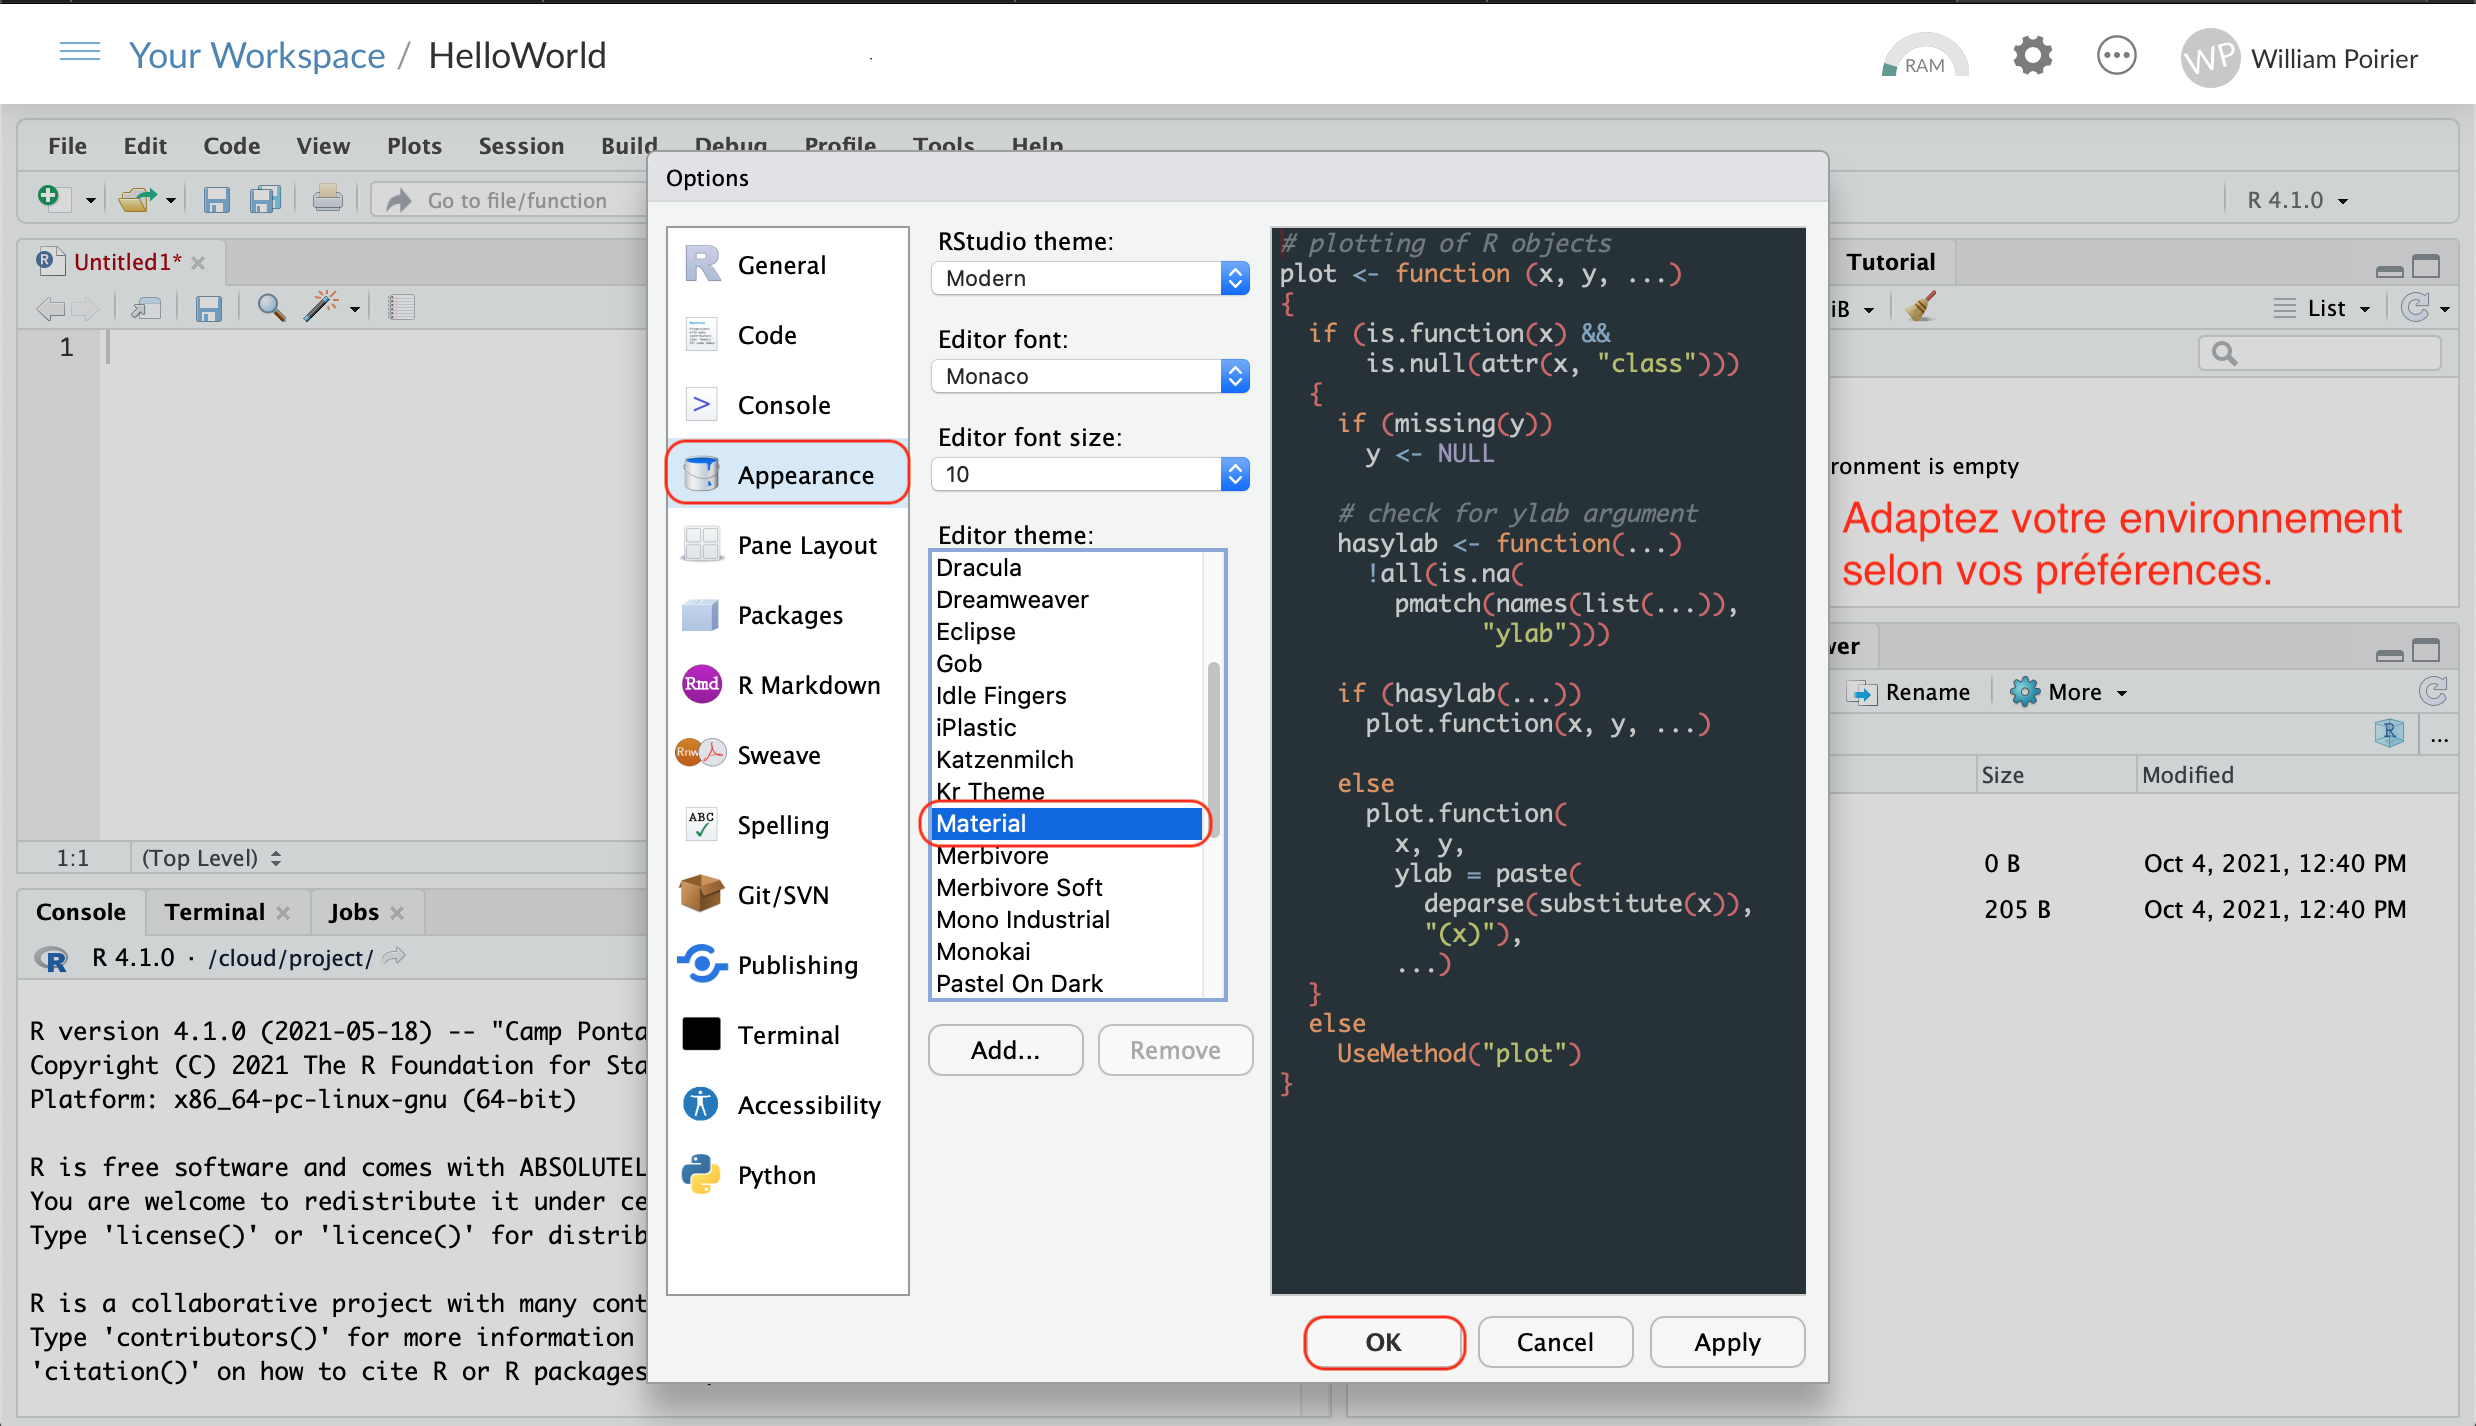
\includegraphics[width=0.98\linewidth]{_graphs/rstudio3.png}}
  \caption{Fin de la personnalisation}
  \label{rstudio3}
\end{figure}

\begin{figure}[H]
  \centering
  \fbox{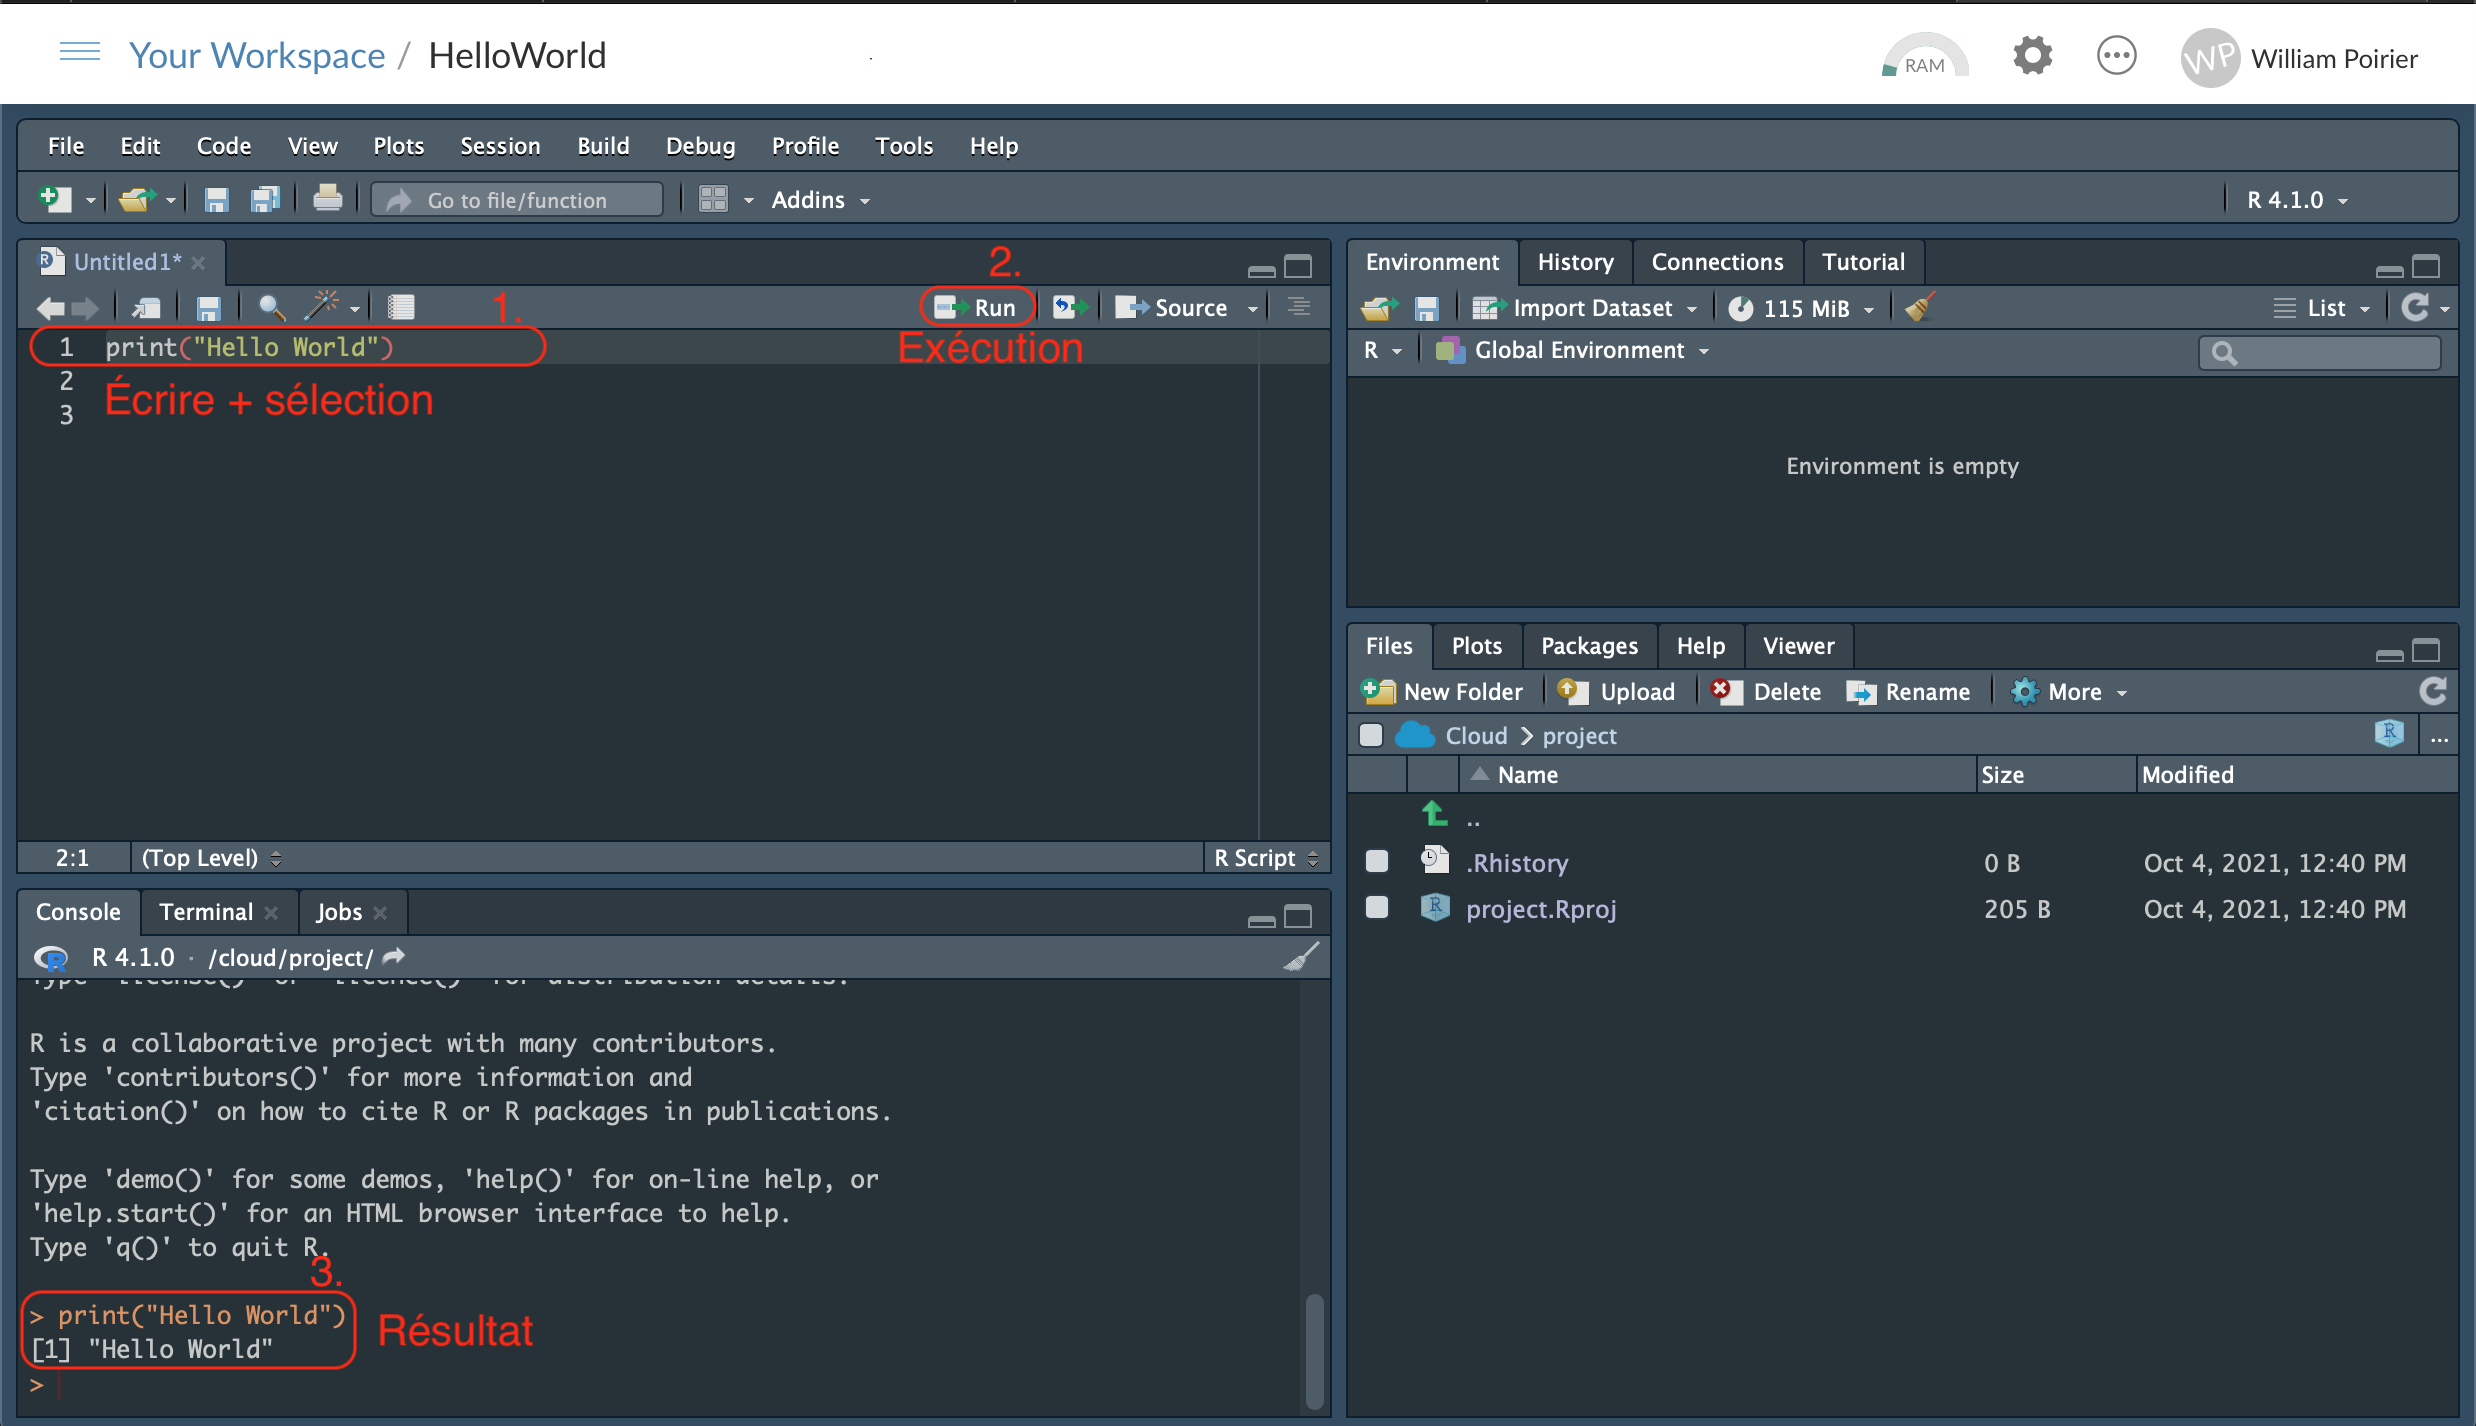
\includegraphics[width=0.98\linewidth]{_graphs/rstudio4.png}}
  \caption{Votre première ligne de code!}
  \label{rstudio4}
\end{figure}


\section{Hello World}

Vous vous apprêtez désormais à écrire votre première ligne de code. Allez dans l'éditeur, et tapez la commande suivante :
\begin{lstlisting}
> print("Hello World")
\end{lstlisting}
À présent, il faut l'exécuter. Pour ce faire, sélectionnez la ligne, puis cliquez sur le bouton \textit{\textbf{RUN}} en haut à droite. La figure \ref{rstudio4} vous montre un exemple. Remarquez que le résultat s'affiche dans la console en bas. C'est sa deuxième utilité. La console vous indique les résultats des commandes que vous exécutez à partir de l'éditeur. Félicitation, vous êtes désormais des programmeurs, le fun peu commencer! 

  \subsection{Workflow}
  
  Un facteur important en prendre en considération lorsque l'on programme ou que l'on gère des bases de données, c'est l'organisation de notre «\emph{flux de travail}». Plusieurs facteurs sont à prendre en considération lorsque l'on veut optimiser son travail. Nous aborderons les principaux dans cette section.
  
    \subsubsection{Arborescence}
    Si vous avez lu le titre de la section et que vous ne savez pas ce à quoi nous faisons référence, ne vous inquiétiez pas, la plupart des gens utilisent l'arborescence de leur ordinateur sans s'en rendre compte. C'est tout simplement le chemin par lequel vous (ou votre ordinateur) doit passer pour accéder à un fichier. Comme quand vous voulez retrouver un vieux travail, votre ordinateur doit connaître où se trouvent les fichiers que vous mobilisez dans votre script. Pour se faire, il faut établir le «répertoire de travail» (\emph{working directory}) de la session \textbf{R}. On utilise alors la fonction \texttt{setwd()} et on y inscrit l'arborescence (le chemin) :
    
    \begin{lstlisting}
    # Pour les Mac
    > setwd("/Users/nomDelaSession/nomDuDossier/nomDuSousDossier")
    # Pour les PC
    > setwd("C:/Users/nomDelaSession/nomDuSousDossier")
    \end{lstlisting}
    
    Remarquez la façon dont l'arborescence est écrit. Chaque dossier est suivi d'une barre oblique (/) et d'un sous-dossier. C'est donc important de bien organiser les dossiers de sorte à éviter de devoir changer de répertoire de travail trop souvent. L'idéal c'est de référer à un dossier général contenant les dossiers spécifiques. Par exemple, vous pourriez avoir un dossier \texttt{ElectionFed21} qui contient un dossier \texttt{codeR}, un dossier \texttt{graphs} et un dossier \texttt{Data}. 
    
    \subsubsection{Commentaires}
    \subsubsection{Raccourcis clavier}
  \subsection{Mathématiques}
    \subsubsection{Calculatrice}
    \subsubsection{Calculatrice+ (table,mean,sd,var etc.}
    \subsubsection{Opérateurs de comparaison}


\section{Intro à la programmation en R}
  \subsection{Ça va bien aller}
  \subsection{L'assignation d'objets}
    \subsubsection{Un peu de vocabulaire}
  \subsection{Les types d'objets}
    \subsubsection{Classes d'éléments}
    \subsubsection{Constante}
    \subsubsection{Vecteurs}
    \subsubsection{Dataframe}
  \subsection{Normes d'assignation - C'est pour votre bien}

  
\section{Importation de données}
  \subsection{Logique de projet RStudio Cloud}
  \subsection{Type de fichier}
  \subsection{Domestication}

  
\section{Analyse - Description}
  \subsection{Univariée}
  \subsection{Bivariée}
  \subsection{Visualisation}


\section{Analyse - Régression}
  \subsection{Linéaire}
  \subsection{Linéaire multiple}

  
\section{Pour aller plus loins}
 
%\section{Bibliographie}
%\begingroup
%\renewcommand{\section}[2]{}
%\bibliographystyle{apacite}
%\bibliography{mybibfile.bib}
%\vspace{10cm}
%\endgroup

\end{document}